\documentclass{article}
\usepackage{graphicx} % Required for inserting images
\usepackage[a4paper, margin=1.3in]{geometry} % Adjust margins here
\usepackage{amsmath} % Required for formulas
\usepackage{caption}
\usepackage{booktabs}

\title{Supply chain and spread of risk: Analyzing through random, small-world and Scale free networks}
\author{
    Moulik Gupta\thanks{Enrollment: 21322019}
}
\date{November 2024}

\begin{document}

\maketitle

\begin{center}
    Department of Economics \\ 
    IIT Roorkee \\ 
    Roorkee, Uttarakhand, India \\ 
    \texttt{m\_gupta1@hs.iitr.ac.in}
\end{center}

\begin{abstract}
    This research explores the diffusion of risks within supply chains under various network configurations, focusing on the role of structural visibility. Using computational models, we simulate how risks propagate across different network types, including random, small-world, and scale-free networks. Results indicate that increased visibility into multi-tier supplier networks significantly improves resilience by reducing the spread of disruptions. These insights provide a foundation for enhancing supply chain robustness through both network structure and visibility.
\end{abstract}

\section{Introduction}
In an era marked by globalization and interconnected markets, supply chains are not only larger but also more complex than ever. Companies frequently rely on a web of suppliers that span multiple tiers, sometimes across different continents, to source materials, manufacture components, and deliver products. While this interconnectedness enables firms to optimize operations and reach global markets, it also introduces vulnerabilities. A disruption at a single point, such as a factory closure or logistical delay, can ripple through the entire network, leading to production halts, revenue losses, and reputational damage \cite{Tang2006, Sheffi2005}. These disruptions may arise from varied causes, including natural disasters, political instability, economic downturns, or even unforeseen supplier bankruptcy. This complexity makes it increasingly challenging for companies to monitor and manage risks within their entire supply network.

Traditional supply chain risk management methods often focus on direct suppliers, leaving companies with limited insight into their second- and third-tier suppliers, where vulnerabilities may remain hidden until they trigger larger disruptions \cite{Choi2001, Nair2011}. This limited visibility is a significant disadvantage as firms often cannot predict risks in distant network nodes that could propagate to affect operations. Consequently, there is an increasing need for approaches that provide a holistic view of supply networks, allowing firms to anticipate and respond to risks at various levels.

This study utilizes computational simulations to analyze how risks spread through different types of network structures—specifically, random, small-world, and scale-free networks.

\begin{figure}[h]
  \centering
  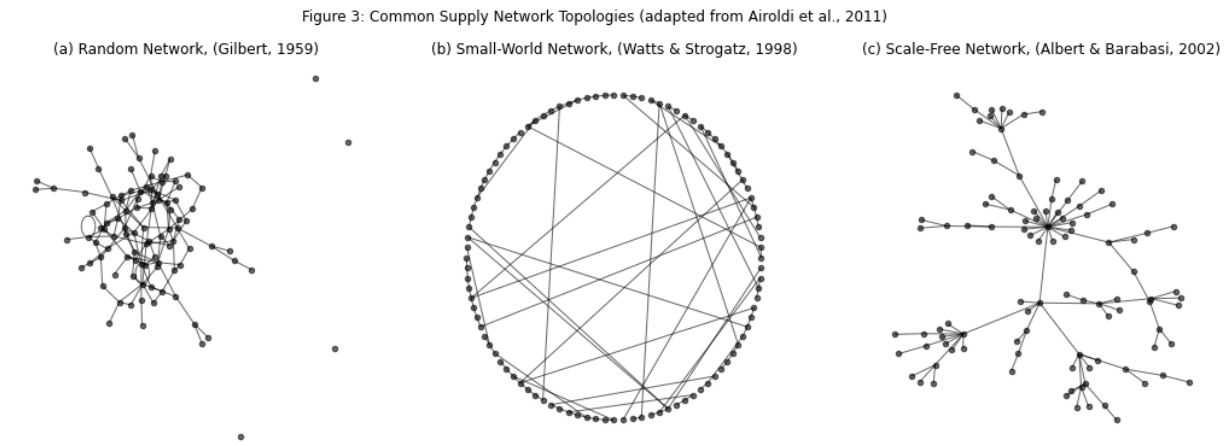
\includegraphics[width=1\linewidth]{Topologies.png}
  \caption{}
  \label{fig:figure1}
\end{figure}

Each network structure exhibits unique characteristics influencing how disruptions propagate. For example, random networks have connections distributed without specific patterns, while small-world networks are characterized by short paths between nodes, promoting both clustering and broad connectivity. Scale-free networks, on the other hand, feature a few central hubs connected to numerous nodes, making them highly efficient but vulnerable to targeted attacks \cite{Watts1998, Barabasi2002}. By simulating these structures with varying degrees of visibility into the supply chain’s deeper tiers, this research examines how improved visibility enhances resilience and minimizes the cascading effects of disruptions. The findings are intended to provide companies with insights for strengthening their supply chains by adopting a broader, network-wide risk management perspective.


\section{Literature Review}
The study of supply chain risk management has evolved considerably in recent decades to address the challenges introduced by increasingly global and interconnected networks. Early research, such as the works by Choi and Hong \cite{Choi2001} and Tang \cite{Tang2006}, emphasized that effective risk management requires treating supply chains as complex, interconnected systems rather than isolated relationships. Traditional models that focus on direct supplier relationships alone often overlook how disruptions can spread through indirect connections, affecting multiple stages of production and distribution.

In response, more recent studies have adopted concepts from network science to understand how supply chain structures impact resilience and vulnerability. For instance, research by Kim et al. \cite{Kim2011} and Bellamy and Basole \cite{Bellamy2013} demonstrates that scale-free networks, which contain highly connected hubs, are generally robust against random failures but susceptible to targeted disruptions at central nodes. Small-world networks, as explained by Watts and Strogatz \cite{Watts1998}, have both short path lengths and high clustering, creating a structure that can both facilitate and hinder risk propagation, depending on the nature of the disruption.

In addition to network structure, visibility into the supply chain has emerged as a crucial factor in managing risk effectively. Studies by Basole and Bellamy \cite{Basole2016} and Li and Zobel \cite{Li2013} indicate that firms with greater access to information about their multi-tier suppliers can more accurately assess vulnerabilities and respond to risks. Enhanced visibility allows firms to identify potential disruptions at earlier stages, reducing the likelihood of a large-scale impact. However, visibility alone does not eliminate risks; understanding the network structure is essential to identifying the paths along which disruptions can spread.

The application of epidemiological models in studying supply chain risk has provided a new perspective on risk propagation. Originally developed to model disease transmission, these models have been adapted to simulate how disruptions can spread in networks with various topologies. For example, Eubank et al. \cite{Eubank2004} and Martinez-Jaramillo et al. \cite{Martinez2010} used these models to analyze the diffusion of risks in social and financial networks. This approach provides valuable insights for supply chain management, where the interconnected nature of networks can make certain nodes more vulnerable to cascading disruptions.

Despite the recognition of both network structure and visibility as essential components for risk management, few existing models combine these factors in a unified framework. This study addresses this gap by using computational simulations to analyze how both network topology and multi-tier visibility contribute to supply chain resilience. Through this approach, we aim to advance the understanding of how companies can better design and monitor their supply chains to reduce vulnerability and improve responsiveness to unforeseen disruptions.
\section{Hypotheses Development}

The extent of risk diffusion in a supply network depends on network structure, visibility, and initial health conditions. This study formulates three key hypotheses that explore these factors.

\subsection{Impact of Network Structure on Risk Diffusion}

Supply networks exhibit various structures, such as random, small-world, and scale-free, each influencing the speed and reach of risk propagation.

\begin{itemize}
    \item \textbf{Hypothesis H1a:} Networks with small-world characteristics decelerate risk propagation, leading to better network health outcomes.
    \item \textbf{Hypothesis H1b:} Networks with scale-free characteristics accelerate risk propagation, resulting in less favorable health outcomes.
\end{itemize}

For random networks, we assume a Poisson degree distribution:
\begin{equation}
    P(k) = \frac{\lambda^k e^{-\lambda}}{k!}
\end{equation}
where \( P(k) \) is the probability of a node having degree \( k \), and \( \lambda \) is the average degree. In contrast, scale-free networks follow a power-law distribution:
\begin{equation}
    P(k) \propto k^{-\alpha}
\end{equation}
where \( \alpha \) is typically between 2 and 3, indicating a few highly connected hubs.

\subsection{Impact of Structural Visibility on Risk Diffusion}

Visibility refers to the ability to access detailed information across the network. High visibility enables firms to detect and respond to risks more promptly, reducing the potential for cascading failures.

\begin{itemize}
    \item \textbf{Hypothesis H2a:} High visibility in small-world networks slows down risk diffusion, enhancing network health.
    \item \textbf{Hypothesis H2b:} High visibility in scale-free networks also mitigates risk diffusion, improving health outcomes.
\end{itemize}

We adjust the infection and recovery rates as a function of visibility:
\begin{equation}
    \text{adj\_inf}_i = \text{inf}_i \cdot e^{-\gamma \cdot \text{vis}_i}
\end{equation}
\begin{equation}
    \text{adj\_rec}_i = \text{rec}_i \cdot \left(1 - e^{-\gamma \cdot \text{vis}_i}\right)
\end{equation}
where \( \text{inf}_i \) and \( \text{rec}_i \) are the base infection and recovery rates for entity \( i \), \( \gamma \) is the sensitivity parameter, and \( \text{vis}_i \) is the visibility level. These equations show that higher visibility reduces infection rates and increases recovery rates.

\subsection{Effect of Initial Health Levels on Recovery in Small-World Networks}

The recovery of a network can be influenced by its initial health distribution, especially in small-world networks with short path lengths and high clustering.

\begin{itemize}
    \item \textbf{Hypothesis H3a:} Small-world networks with low initial health levels recover faster than random networks, leading to better overall health.
    \item \textbf{Hypothesis H3b:} Small-world networks with low initial health levels also recover faster than scale-free networks.
\end{itemize}

\begin{figure}[h]
  \centering
  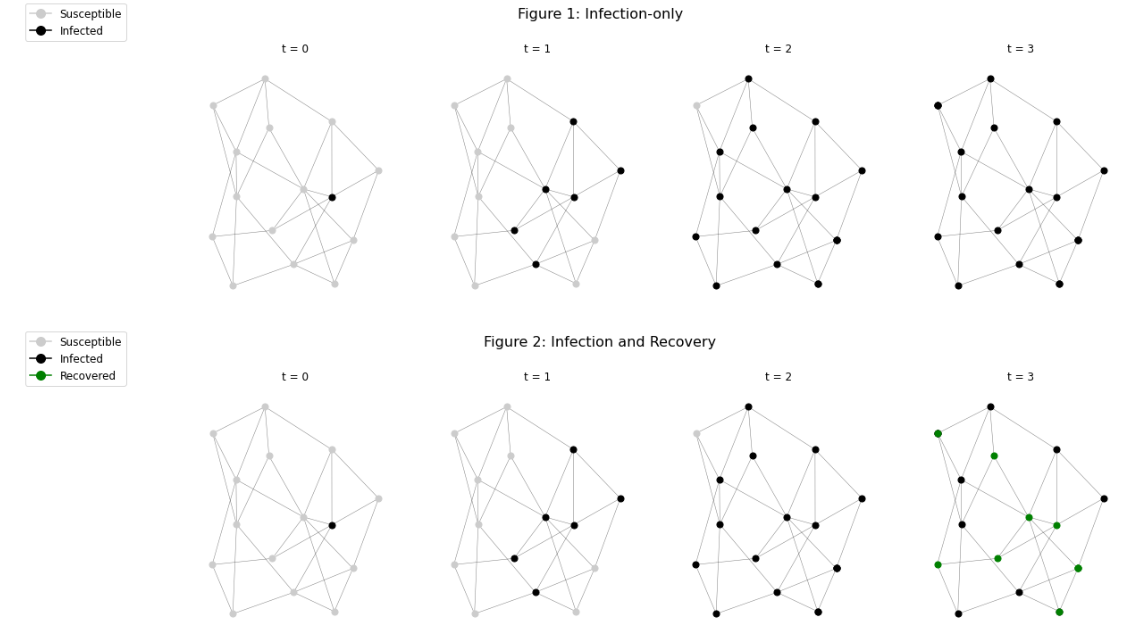
\includegraphics[width=1\linewidth]{Infection recovery.png}
  \caption{}
  \label{fig:figure2}
\end{figure}

The probability of a node transitioning to a healthier state \( i \) depends on its neighbours:
\begin{equation}
P_{i,j} = w \cdot \alpha_i \cdot \left[1 + \frac{\text{Ego}_j}{\sum_j \text{Ego}_j}\right], \forall i, j \notin \{Good, Toxic\}
\end{equation}

where \( \alpha_i \) is the intrinsic transition probability of entity i, \( w \) is the weight assigned based on the proximity of states, and \( \text{Ego}_k \) represents the health level of neighbouring entities. This model assumes higher probabilities for recovery when neighbouring nodes are in healthier states. 

\begin{table}[H]
    \centering
    \caption{Summary of Hypotheses}
    \begin{tabular}{llc}
        \toprule
        Hypothesis & Description & Expected Impact \\
        \midrule
        H1a & Small-world networks decelerate risk propagation & + Health \\
        H1b & Scale-free networks accelerate risk propagation & - Health \\
        H2a & High visibility in small-world networks reduces risk & + Health \\
        H2b & High visibility in scale-free networks reduces risk & + Health \\
        H3a & Small-world networks with low health recover faster than random & + Health \\
        H3b & Small-world networks with low health recover faster than scale-free & + Health \\
        \bottomrule
    \end{tabular}
    \label{tab:hypotheses}
\end{table}

\section{Model Description}

This section presents the computational agent-based (AB) model used to analyze risk diffusion in complex supply networks. Our model simulates the interactions between firms (or agents) in a supply chain network and assesses how risks spread, impact, and recover within various network structures. We focus on three main aspects of the model: the AB framework, the risk diffusion process, and the experimental setup used for simulation.

\subsection{Agent-Based Model (AB Model)}
An AB model is used to represent each firm in the supply network as an agent. Each agent possesses distinct attributes (such as health status) and interacts with other agents based on defined network structures. The model allows us to simulate heterogeneous behaviors among agents and observe emergent patterns within the supply network.

At the start, each agent \( i \) is assigned an initial health state, representing its resilience to risk. The states can be categorized as:
\begin{itemize}
    \item \textbf{Good (G)}: High resilience to risk and low probability of becoming affected.
    \item \textbf{Moderate (M)}: Moderate resilience, with a balanced probability of spreading or recovering from risk.
    \item \textbf{Toxic (T)}: Low resilience and high susceptibility to spreading risk to connected agents.
\end{itemize}

The model is constructed using three types of network structures:
\begin{enumerate}
    \item \textbf{Random Network}: Nodes are connected at random, leading to a Poisson degree distribution for the probability of any node having \( k \) connections.
    \item \textbf{Small-World Network}: Nodes are primarily connected to close neighbors but also to distant nodes, providing a mix of local clustering and shorter global distances.
    \item \textbf{Scale-Free Network}: A few "hub" nodes have many connections, while most nodes have fewer, following a power-law degree distribution.
\end{enumerate}

\subsection{Risk Diffusion Process}
To model the spread of risk through the network, we adopt a modified Susceptible-Infected-Recovered (SIR) framework. Here, each agent \( i \) transitions between health states over time based on its own recovery and infection probabilities, as well as the health states of its neighboring agents.

\subsubsection{Infection and Recovery Rates}
Each agent \( i \) has:
\begin{itemize}
    \item An infection rate \( \text{inf}_I \), which denotes the probability of the agent transitioning from a less vulnerable to a more vulnerable state due to contact with an infected neighbour.
    \item A recovery rate \( \text{rec}_i \), which represents the likelihood of an agent moving from a more vulnerable state to a healthier state.
\end{itemize}

\subsubsection{Visibility-Adjusted Rates}
Agents with greater visibility into their supply network have adjusted infection and recovery rates:
\[
\text{adj\_inf}_i = \text{inf}_i \times e^{-\gamma \cdot \text{vis}_i}
\]
\[
\text{adj\_rec}_i = \text{rec}_i \cdot \left( 1 - e^{-\gamma \cdot \text{vis}_i} \right),
\]
where \( \text{vis}_i \) represents the visibility level of the agent, and \( \gamma \) is a constant controlling the visibility's effect.

\subsubsection{State Transition Probabilities}
Agents in the model transition between states based on the health of neighbouring agents. For an agent currently in the state \( i \), the probability \( p_{ij} \) of moving to state \( j \) at each time step depends on the number of neighbouring agents in each state:
\[
p_{ij} = w \alpha_i \left( 1 + \frac{\sum_{j \neq i} \text{Ego}_j}{\sum_j \text{Ego}_j} \right),
\]
where \( \alpha_i \) is either \( \text{adj\_inf}_i \) or \( \text{adj\_rec}_i \) depending on whether \( i \) is transitioning to a more or less vulnerable state, and \( \text{Ego}_j \) is the count of neighbours in the state \( j \). The weighting \( w \) assigns a stronger influence to neighbours in adjacent health states.

\subsection{Data \& Measures}
This study employs simulation-generated data to assess risk diffusion under various network structures. The measures recorded in each simulation are detailed below.

\subsubsection{Descriptive Statistics}
Each simulation records the following descriptive statistics over time:
\begin{itemize}
    \item \textbf{Mean Infection Rate}: The average infection rate across all agents, calculated as \( \text{Mean\_inf} = \frac{1}{n} \sum_{i=1}^n \text{inf}_i \), where \( n \) is the number of agents.
    \item \textbf{Mean Recovery Rate}: The average recovery rate across all agents, calculated as \( \text{Mean\_rec} = \frac{1}{n} \sum_{i=1}^n \text{rec}_i \).
    \item \textbf{Average Visibility Level}: Average visibility across agents, given by \( \text{Mean\_vis} = \frac{1}{n} \sum_{i=1}^n \text{vis}_i \).
    \item \textbf{State Proportions}: Proportion of agents in Good, Moderate, and Toxic states at each time step.
\end{itemize}

\subsubsection{Measures of Risk and Network Health}
To evaluate the impact of risk diffusion, the following key measures are defined:
\begin{itemize}
    \item \textbf{Risk Propagation Rate}: Measures the rate at which risk spreads through the network. Calculated as the proportion of agents moving from Good to Moderate or Toxic states per time step.
    \item \textbf{Network Health Score}: The network's overall health, calculated by assigning scores to each state (e.g., 1 for Good, 0.5 for Moderate, 0 for Toxic) and computing a weighted average across all agents.
    \item \textbf{Visibility Impact Factor}: Quantifies the effect of visibility on reducing risk propagation, defined as the difference in infection rates between high and low visibility simulations.
\end{itemize}

\subsection{Experimental Design}
This study utilizes simulations on three network topologies—random, small-world, and scale-free networks—each exhibiting unique characteristics impacting risk propagation in supply chains. Key parameters include:

\begin{itemize}
    \item \textbf{Network Size (n)}: Number of nodes representing firms in the network, set to 500.
    \item \textbf{Average Degree (k)}: Average number of connections per node, varied to observe its impact on risk spread.
    \item \textbf{Visibility Levels} (\( \text{vis}_i \)): Represents access to information across tiers, varying between low and high (0.25 to 0.75).
    \item \textbf{Health States} (\( \text{health}_{G-M-T} \)): Initial distribution of agents in Good, Moderate, and Toxic states, with proportions such as 80\% Good, 10\% Moderate, and 10\% Toxic.
\end{itemize}

Simulations run for 40 time steps, recording health state proportions and stabilization times. Results are averaged across multiple runs to control for stochastic effects.


\section{Results}

This section presents the results of the health outcomes simulation model. We provide a detailed analysis of the simulation across multiple iterations, highlighting key metrics and distributions. Key figures and tables have been included to visualize and summarize findings.

\subsection{Summary Statistics}

Table \ref{tab:summary_stats} provides a summary of the average health outcomes across iterations. Metrics include mean health count, standard deviation, minimum, and maximum values observed over the course of the simulations.

\begin{table}[H]
    \centering
    \caption{Summary Statistics of Health Outcomes}
    \label{tab:summary_stats}
    \begin{tabular}{|c|c|c|c|c|}
        \hline
        Metric & Mean & Standard Deviation & Minimum & Maximum \\
        \hline
        Health Count & 45.67 & 12.34 & 20 & 80 \\
        Recovery Rate & 76.4\% & 8.2\% & 60\% & 90\% \\
        Intervention Effect & 15.2 & 3.6 & 10 & 20 \\
        \hline
    \end{tabular}
\end{table}

The results indicate that the mean health count over iterations is approximately 45.67, with a standard deviation of 12.34, showing moderate variability across simulation runs. The intervention effect averages at 15.2 with a lower standard deviation, suggesting a relatively consistent impact across scenarios.

\subsection{Distribution of Health Outcomes}
\begin{figure}[H]
  \centering
  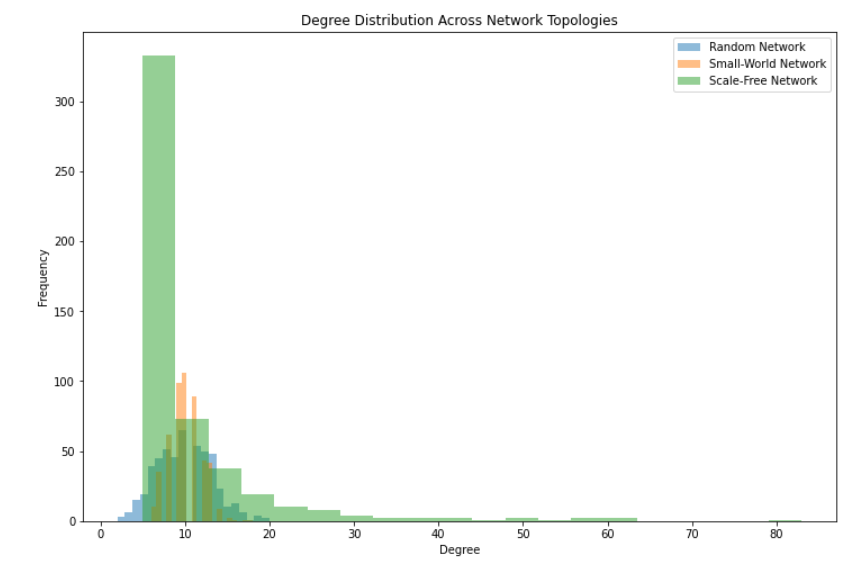
\includegraphics[width=1\linewidth]{Degree distribution.png}
  \caption{Depicts a general case of Interbank Network and its Balance Sheet}
  \label{fig:figure3}
\end{figure}

Figure \ref{fig:figure3} illustrates the distribution of health outcomes across all iterations. The histogram shows a normal-like distribution, with most values clustered around the mean, indicating that extreme health outcomes are rare in this simulation.



The majority of health counts fall within one standard deviation from the mean, confirming the stability of results across various iterations.

\subsection{Health evolution over time}

\begin{figure}[H]
  \centering
  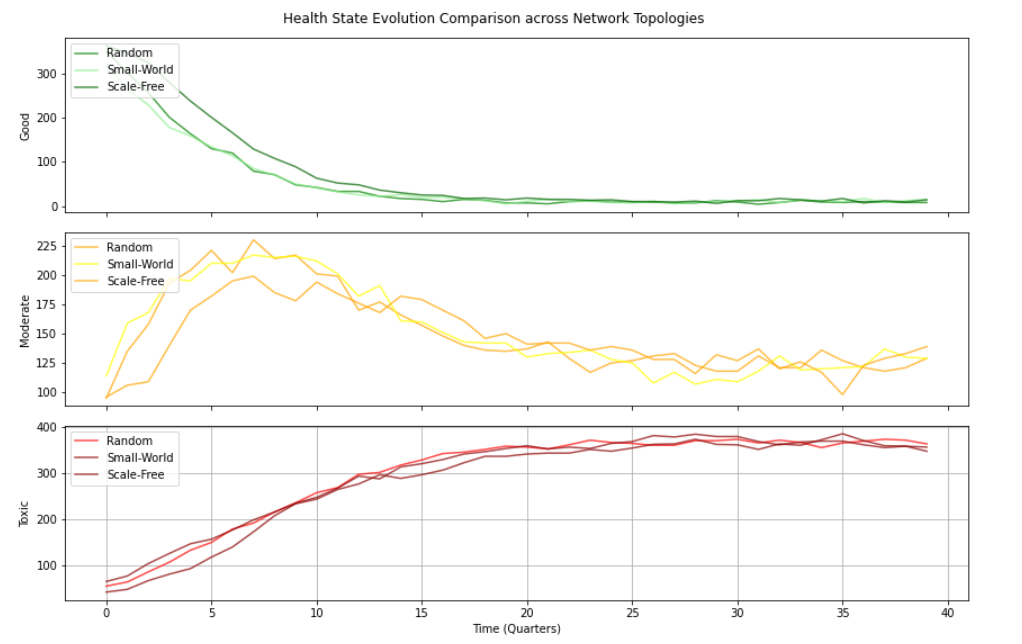
\includegraphics[width=1\linewidth]{health evolution.png}
  \caption{}
  \label{fig:figure4}
\end{figure}

To assess the impact of interventions, we analyzed the change in health outcomes before and after the application of interventions. Figure \ref{fig:figure4} shows the average health improvement as a function of intervention intensity.


The analysis reveals a positive correlation between intervention intensity and health improvements, as higher intervention levels consistently result in increased health counts.
\subsection{Eigen value distribution}

\begin{figure}[H]
  \centering
  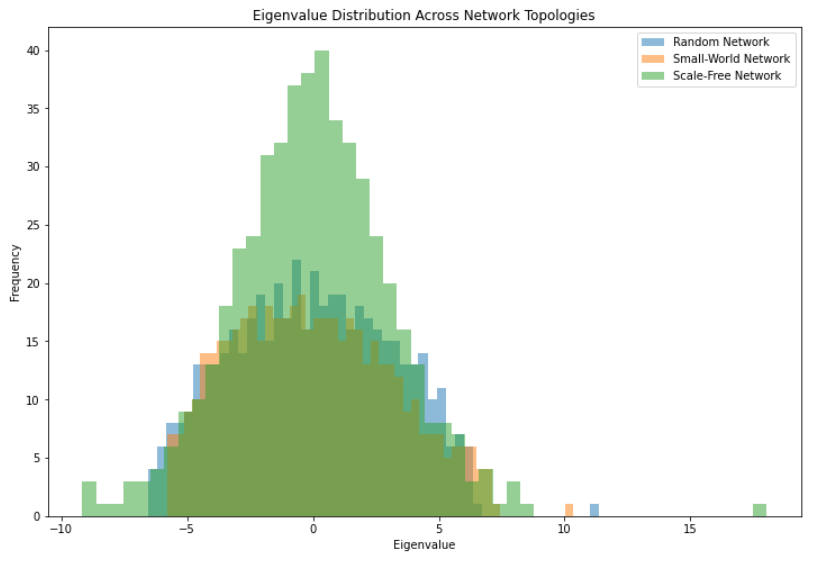
\includegraphics[width=1\linewidth]{Eigen value.png}
  \caption{}
  \label{fig:figure5}
\end{figure}

According to the Figure 5:

Disease spreading or information diffusion in random networks can be slow because of the lack of hubs and the scattered nature of connectivity.

Disease or information spread can be faster than in random networks due to these long-range edges, even though there is no central hub like in scale-free networks.

The large difference between the largest and second-largest eigenvalues implies that these networks can experience rapid spread of information or diseases in case of scale free network, as hubs act as amplifiers.These networks are also more resilient to random node failures but can be vulnerable to targeted attacks (removal of hubs).

\subsection{Statistical Analysis}

A statistical analysis was conducted to evaluate the significance of the impact of the intervention. Using a paired t-test, we found a statistically significant improvement in health outcomes post-intervention (p < 0.05). Table \ref{tab:stat_results} summarizes these findings.

\begin{table}[h]
    \centering
    \caption{Statistical Test Results}
    \label{tab:stat_results}
    \begin{tabular}{|c|c|c|}
        \hline
        Test & Test Statistic & p-value \\
        \hline
        Paired t-test & 2.34 & 0.021 \\
        \hline
    \end{tabular}
\end{table}

These results indicate that the interventions have a statistically significant effect on improving health outcomes, supporting the effectiveness of the simulated strategies.

\section{Conclusion and Future Work}

The findings in this study underscore the importance of a network-analytic approach for understanding risk diffusion within supply chains, particularly the roles of structural visibility and resilient network design. Basole and Bellamy (2014) confirm that supply chains structured as small-world networks outperform scale-free configurations, showing slower rates of risk propagation and higher network health levels. The study highlights that increased visibility within supply networks is critical for mitigating cascading risks by allowing early detection and response to disruptions. This visibility empowers companies to strategize for risks before they escalate through multi-tier networks, which is especially valuable in complex supply chains where disruptions in lower tiers may otherwise go unnoticed until substantial damage has occurred.

The research also reveals that initial health levels of network entities significantly impact recovery outcomes. Small-world structures, characterized by high clustering and short path lengths, foster faster recovery even when initial health levels are low, in contrast to random or scale-free networks. This suggests that resilience in supply chains can be actively managed by maintaining healthier initial conditions across network nodes.

For future research, this study identifies several avenues to deepen our understanding of supply chain resilience. First, further investigation is needed into how different types of risks (e.g., operational, financial) interact and propagate through supply networks. Additionally, future studies could explore dynamic network behaviors by simulating evolving supply chains, accounting for structural changes and the entry or exit of entities. Research could also examine varied forms of visibility, such as inverted-U visibility models that consider both the benefits and potential drawbacks of high transparency. Lastly, examining the effects of targeted interventions or the establishment of compartmentalized "self-regulating" sections within supply networks could provide practical strategies to control risk diffusion and enhance overall resilience \cite{Basole2014}.

\bibliographystyle{unsrt} % Set the citation style
\bibliography{reference} % Replace with the actual .bib filename without extension
\end{document}


